\documentclass{cours}
\usepackage{esvect}
\usepackage{pgfplots}
\usepackage{multicol}
\usepackage{amssymb}
\usepackage{tikz-3dplot}
\usepackage{xr}
\usepackage{fontawesome}
\usetikzlibrary {decorations.text, backgrounds, intersections}

\begin{document}

\setcounter{chapter}{23}
\chapter{Actions d'un champ magnétique}
Dans tout ce chapitre, nous considérerons que je champ magnétique est \emph{uniforme} et \emph{stationnaire}.

\section{Sur un fil, rails de Laplace}%
\label{sec:sur_un_fil}
On observe que lorsqu'on place un fil conducteur parcouru par un courant électrique dans un champ magnétique, il subit une force perpendiculaire au conducteur et au champ magnétique.

\subsection{Résultante}%
\label{sub:resultante}

Un petit élément orienté $\vv{\mathrm{d}\ell}$ du fil parcouru par un courant $i$  subit une force :
\begin{equation}
  \vv{\mathrm{d}F} = i\vv{\mathrm{d}\ell} \wedge \vv{B}
\end{equation}
\begin{center}
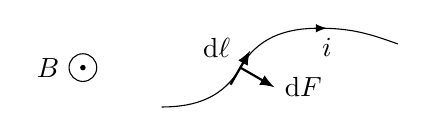
\begin{tikzpicture}
%tikz magnetisme  
  \draw (0,0) to[out=0, in=-120] (1,0.5) to[out=60, in=180] (2, 1) to[out=0, in=160] (3,0.8);
  \draw[thick, -latex] (1, 0.5) ++(60:-0.25) -- ++(60:0.5) node[midway, above left]{$\vv{\mathrm{d}\ell}$}; 
  \draw[-latex] (2,1) -- ++(0.1,0) node[below]{$i$ };
  \draw[-latex, thick] (1, 0.5) -- ++(-30:0.5) node[right]{$\vv{\mathrm{d}F}$ }; 
  \fill (-1, 0.5) circle (1pt);
  \draw (-1, 0.5) circle (5pt);
  \draw (-1, 0.5) ++ (-5pt, 0) node[left]{$\vv{B}$};
\end{tikzpicture}

\captionof{figure}{Force de Laplace subie par un petit élément de longueur d'un fil parcouru par un courant $i$.}
\end{center}
$\vv{B}$ est le champ magnétique extérieur, c'est à dire le champ magnétique créé par les sources autres que l'élément $\vv{\mathrm{d}\ell}$. Fondamentalement, la force de Laplace n'est qu'une conséquence de la force de Lorentz qui s'exerce sur les porteurs de charge (électrons) qui se déplacent pour provoquer le courant $i$. On avait vu que la force de Lorentz magnétique subie par une charge $q$ se déplaçant avec une vitesse $\vv{v}$ dans un champ magnétique $\vv{B}$ était 
\begin{equation}
  \vv*{F}{L} = q\vv{v}\wedge \vv{B}
\end{equation}

Donc la force totale subie par la portion de conducteur de longueur $\vv{\mathrm{d}\ell}$ sera 
\begin{equation}
  \vv{\D F} = N \vv*{F}{L} = nS\D \ell q \vv{v} \wedge \vv{B}\, ,
\end{equation}
où 
\begin{itemize}
  \item $N$ est le nombre d'électrons dans la portion de circuit considérée ;
  \item $n$ est le nombre d'électrons par unité de volume dans le conducteur ;
  \item $S$ est la section du conducteur 
\end{itemize}
En notant que $nSqv = i$, et en remarquant que les vecteurs $\vv{\D\ell}$ et $\vv{v}$ sont colinéaires, on obtient bien l'expression de la force de Laplace
\begin{eqencadre}
  \vv{\D F} = i\vv{\D \ell} \wedge \vv{B}
\end{eqencadre}

On peut appliquer ce résultat à l'expérience des rails de Laplace : une barre mobile posée sur deux rails fixes parallèles est parcourue par un courant $i$. Le champ magnétique extérieur est uniforme et perpendiculaire à la barre.
\begin{center}
  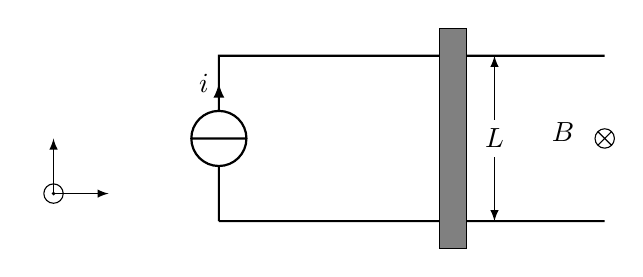
\begin{tikzpicture}[scale=0.7]
  %tikz magnetisme
    \coordinate (A) at (-1, 0.5);
    \draw[-latex] (A) -- ++(1,0) node[right]{$\vex $} ;
    \draw[-latex] (A) -- ++(0,1) node[left]{$\vey $} ;
    \fill (A) circle(1pt);
    \draw (A) circle(5pt);
    \draw (A) ++ (-135:5pt) node[below left]{$\vez $}; 
    
    \coordinate (B) at (2,0);
    \draw[thick] (B) -- ++(0, 1) ++(0,1) -- ++(0,1) -- ++(7, 0)
                 (B) -- ++(7,0)
                 (B) ++ (0,1.5) circle(0.5)
                 (B) ++(-0.5, 1.5) -- ++(1,0);
    \draw[fill=gray] (B) ++(4,-0.5) rectangle ++(0.5, 4);
    \draw[latex-latex] (B) ++(5, 0) -- node[fill=white]{$L$ } ++(0,3);
    \draw[thick, -latex] (B) ++(0,2) -- ++(0,0.5) node[left]{$i$ };
    \draw (B) ++(7,1.5) circle (5pt)
          +(45:5pt) -- +(-135:5pt)
          +(-45:5pt) -- +(135:5pt)
          node[left, xshift=-5pt]{$\vv{B}$};
  \end{tikzpicture}
  \captionof{figure}{Expérience des rails de Laplace. Une barre conductrice mobile est placée sur deux rails conducteurs parcourus par un courant $i$ dans un champ magnétique $\protect\vv{B}$. }
\end{center}
La force subie par la barre est 
\begin{equation}
  \vv{F} = \int \vv{\D F} = \int i \vv{\D \ell} \wedge \vv{B}  
\end{equation}
%
Comme $\vv{B}$ est uniforme, on peut le sortir de l'intégrale, ainsi que $i$, on obtient alors 
\begin{equation}
  \vv{F} =  i\left(\int \vv{\D \ell}\right) \wedge \vv{B} = iL(-\vey)\wedge (-B \vez) = iLB \vey \wedge \vez  = iLB \vex
\end{equation}
Pour connaitre la direction et le sens de $\vv{F}$, on peut utiliser la \emph{règle de la main droite} (encore elle !) :
\begin{center}
  \def\svgwidth{6cm}
  \input{images/regle_main_droite2.pdf_tex}
  
  \captionof{figure}{Règle de la main droite pour déterminer sans calcul la direction et le sens de la force de Laplace}
\end{center}

\subsection{Puissance}%
\label{sub:puissance}
Dans l'expérience des rails de Laplace, la puissance de la force de Laplace est 
\begin{equation}
  P_\text{Laplace} = \vv*{F}{\text{Laplace}} \cdot \vv{v}
\end{equation}
où $\vv{v}$ est la vitesse du point d'application de la force, ici il s'agit de la vitesse de la barre $\vv{v} = v \vex $. 
On a donc 
\begin{equation}
  P_\text{Laplace} = iLBv = iB \dt{S}\, ,
\end{equation}
où $\dt{S}$ est l'aire balayée par la barre par unité de temps. On peut noter $\phi = BS$ (c'est le flux du champ magnétique à travers le circuit, on le définira plus tard). La puissance de la force de Laplace est alors :
\begin{equation}
  P_\text{Laplace} = i\dt{\phi}
  \label{eq:puissance}
\end{equation}

\section{Sur une spire}%
\label{sec:sur_une_spire}

On considère une spire de courant rectangulaire plongée dans un champ magnétique uniforme. La spire est libre de tourner autour d'un axe passant par les milieux de deux côtés opposés.
\begin{center}
\tdplotsetmaincoords{70}{40}
\begin{tikzpicture}[tdplot_main_coords]
%tikz magnetisme
  \tikzset{axe/.style={-latex, thick, gray}}
  \draw[axe] (-1,0,0) -- (7,0,0) node[right, color=black]{$x$};
  \draw[axe] (0,-3,0) -- (0,3,0) node[above, color=black]{$y$};
  \draw[axe] (0,0,-3) -- (0,0,3) node[above, color=black]{$z$};
  \draw[tdplot_main_coords](0,0,0) node[left]{$O$ };
  \tdplotsetrotatedcoords{90}{-45}{0}
  \draw[line width=3pt, white, tdplot_rotated_coords](-2, 0, 0) -- (-2, -4, 0);
  \draw[thick, tdplot_rotated_coords](-2,0,0)  node[below left](A){$A$}-- (2, 0, 0)  node[above left](D){$D$}-- (2, -6, 0) node[above right](C){$C$}  -- (-2, -6, 0) node[below](B){$B$}  -- cycle;
  \draw[latex-latex] (A.east) -- node[fill=white, inner sep=2pt]{$\ell$} (B.west);
  \draw[latex-latex, tdplot_rotated_coords] (-2, -6.5, 0) -- node[pos=0.3,fill=white, inner sep=2pt]{$L$} (2, -6.5, 0);
  \draw[thick, tdplot_rotated_coords, -latex] (0, 0, 0) -- (-1, 0, 0) node[left]{$i$}; 
  \draw[tdplot_main_coords, -latex, thick] (9, 0, 0) -- ++(0,0, 1) node[midway, right]{$\vv{B} = B \vez $ }; 
   \tdplotsetthetaplanecoords{90}
   \tdplotdrawarc[tdplot_rotated_coords, -latex]{(0,0,0)}{1.5}{90}{45}{right}{$\theta$};
  \end{tikzpicture}
  \captionof{figure}{Spire de courant rectangulaire plongée dans un champ magnétique uniforme.}
\end{center}
\subsection{Résultante}%
\label{sub:resultante}
La résultante des forces de Laplace appliquées à la spire est 
\begin{align}
  \vv*{F}{\text{Laplace}} &= \vv*{F}{AB} +  \vv*{F}{BC} + \vv*{F}{CD} + \vv*{F}{DA} \\
   &= i\vv{AB}\wedge \vv{B} + i\vv{BC}\wedge \vv{B} +i\vv{CD}\wedge \vv{B} +i\vv{DA}\wedge \vv{B}\\
   &=i\underbrace{(\vv{AB}+\vv{BC}+\vv{CD}+\vv{DA})}_{=0}\wedge \vv{B} = \vv{0}
\end{align}
On en déduit que la résultante des forces de Laplace qui s'exercent sur la spire est nulle. On généralise ce résultat à n'importe quel moment magnétique.
\begin{loi}{Moment magnétique dans un champ magnétique uniforme}
  La résultante des forces de Laplace appliquées à un moment magnétique plongé dans un champ magnétique uniforme est nulle
\end{loi}

\subsection{Couple}%
\label{sub:couple}
La résultante étant nulle, les forces de Laplace produisent un \emph{couple} $\vv*{\Gamma}{\text{Laplace}}$ sur la spire :
\begin{equation}
  \vv*{\Gamma}{\text{Laplace}} = \vv*{\mathcal{M}}{O}(\vv*{F}{AB}) + \vv*{\mathcal{M}}{O}(\vv*{F}{BC}) + \vv*{\mathcal{M}}{O}(\vv*{F}{CD}) + \vv*{\mathcal{M}}{O}(\vv*{F}{DA})   
\end{equation}
Par ailleurs, on remarque que les forces appliquées sur les sections $AD$ et $BC$ ont leur point d'application sur l'axe $Ox$ et sont dirigées suivant $\vex $. La droite qui porte ces forces passe donc par le point $O$ et le moment de ces forces par rapport à $O$ est nul :

\begin{equation}
  \vv*{\mathcal{M}}{O}(\vv*{F}{BC}) +\vv*{\mathcal{M}}{O}(\vv*{F}{DA}) = \vv{0}
\end{equation}

Il reste à déterminer les moments des deux forces restantes :
\begin{equation}
  \vv*{F}{AB}  = i\vv{AB}\wedge \vv{B} = i\ell \vex  \wedge B \vez  = -i\ell B \vey = -\vv*{F}{BC}
\end{equation}

Le couple de forces appliquées à la spire est (voir cours correspondant)
\begin{align}
  \vv*{\Gamma}{\text{Laplace}} &=\vv{DA}\wedge \vv*{F}{AB} = \vv{DA} \wedge \left( -i\vv{AB} \wedge \vv{B} \right)  = -\vv{DA} \wedge \left( i\vv{AB} \wedge \vv{B} \right) \\
  &=i\underbrace{\vv{AB} \wedge \left( \vv{B} \wedge \vv{DA} \right)}_{\vv{0}} + i\vv{B}\wedge \left( \vv{DA}\wedge \vv{AB} \right)\\
  &=i\underbrace{\left( \vv{AD} \wedge \vv{AB} \right)}_{\vv{S}} \wedge\vv{B} = \vv{\mu} \wedge \vv{B}
\end{align}
Donc le couple de forces subi par un moment magnétique $\vv{\mu}$ plongé dans un champ magnétique uniforme $\vv{B}$ est 
\begin{eqencadre}
  \vv{\Gamma} = \vv{\mu} \wedge \vv{B}
\end{eqencadre}

\subsection{Puissance}%
\label{sub:puissance}
La puissance fournie par les forces de Laplace est $P=\Gamma_\text{Laplace}\times \omega $, où $\omega=\dot{\theta}$ est la vitesse angulaire de la spire (ou de l'aimant). 

On peut écrire $P$ comme
\begin{equation}
  P = -i\ell L B \sin(\theta) \dot{\theta} = \dt{iSB\cos(\theta)}\, .
\end{equation}
En notant $\phi=SB\cos(\theta)$ le flux du champ magnétique à travers la surface $S$, on retrouve la même expression que~\ref{eq:puissance} pour la puissance des forces de Laplace.  

\section{Sur un aimant permanent}%
\label{sec:sur_un_aimant_permanent}

\subsection{Actions mécaniques}%
\label{sub:actions_mecaniques}

Un aimant permanent peut être assimilé à un moment magnétique $\vv{\mu}$, les résultats que nous avons obtenus dans la partie~\ref{sec:sur_une_spire} restent valables :
\begin{itemize}
  \item La résultante des forces magnétiques est nulle $\vv{F}=\vv{0}$ ;
  \item Le couple appliqué par les forces magnétiques est $\vv{\Gamma}=\vv{\mu}\wedge \vv{B}$, et $\norm{\vv{\Gamma}} = \norm{\vv{\mu}} \norm{\vv{B}} \sin(\theta)$. Où $\theta$ est l'angle entre $\vv{\mu}$ et $\vv{B}$.    
\end{itemize}
\begin{center}
  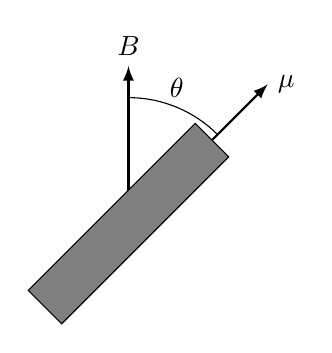
\begin{tikzpicture}
  %tikz magnetisme
    \draw[thick, -latex] (0,0) -- ++(0,2) node[above] {$\vv{B}$ };
    \draw (45:1.6) arc(45:90:1.6) node[midway, above]{$\theta$}; 
    \draw[rotate=45, fill=gray] (-1.5, 0.3) rectangle (1.5,-0.3);  
    \draw[-latex, thick] (45:1.5) -- ++(45:1) node[right]{$\vv{\mu}$};
  \end{tikzpicture}
  \captionof{figure}{Moment magnétique dans un champ magnétique uniforme.}
\end{center}
\subsection{Énergie potentielle}%
\label{sub:energie_potentielle}

On a vu que la puissance des forces magnétiques est $P=\dt{}\left(iSB\cos(\theta)\right)$, donc on peut écrire cette puissance comme
\begin{equation}
  P = \dt{\left(\vv{\mu}\cdot \vv{B}\right) } = -  \dt{E_p}\, , 
\end{equation}
par définition de l'énergie potentielle associée à une force conservative. L'énergie potentielle d'un moment magnétique $\vv{\mu}$ plongé dans un champ magnétique uniforme $\vv{B}$ est donc 
\begin{eqencadre}
  E_p = -\vv{\mu}\cdot\vv{B} = -\mu B \cos(\theta)
\end{eqencadre}
où $\mu=\norm{\vv{\mu}}$, $B=\norm{\vv{B}}$ et $\theta$ est l'angle entre $\vv{\mu}$ et $\vv{B}$.    

On peut tracer un graphe d'énergie potentielle en fonction de $\theta$ :

\begin{center}
  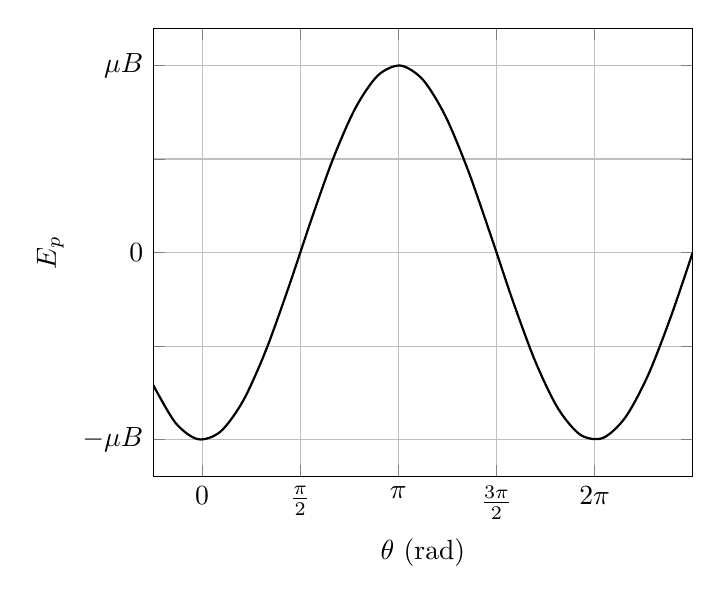
\begin{tikzpicture}
  %tikz magnetisme
    \begin{axis}[
    grid=major,
    xlabel=$\theta$ (rad),
    ylabel=$E_p$,  
    xmin=-45, xmax=450,
    xtick={0,90, 180, 270, 360},
    xticklabels={$0$, $\frac{\pi}{2}$, $\pi$, $\frac{3\pi}{2}$, $2\pi$},  
    ytick={-1, -0.5, 0, 0.5, 1},
    yticklabels={$-\mu B$, $ $, $0$, $ $, $\mu B$},
    ]
      \addplot[domain=-45:450, smooth, thick]{-cos(x)};
    \end{axis}
  \end{tikzpicture}
\captionof{figure}{Énergie potentielle d'un moment magnétique plongé dans un champ magnétique uniforme en fonction de l'angle $\theta$ entre le champ magnétique et le moment. }
\end{center}
Sur ce graphe, on observe que :
\begin{itemize}
  \item Les angles $\theta\equiv 0 \mod 2\pi$ sont des minima d'énergie potentielle, ils correspondent à des \textbf{positions d'équilibre stables}, le moment magnétique est aligné avec le champ magnétique.
\item Les angles $\theta \equiv \pi \mod 2\pi$ sont des maxima d'énergie potentielle, ils correspondent à des \textbf{positions d'équilibre instables}, le moment magnétique et le champ magnétique pointent dans des directions opposées.
\end{itemize}

\subsection{Application : effet moteur d'un champ magnétique tournant}%
\label{sub:application_effet_moteur_d_un_champ_magnetique_tournant}

On a vu qu'un moment magnétique a tendance à s'aligner avec le champ magnétique. Si on produit un champ magnétique dont l'orientation tourne au cours du temps, on peut mettre en rotation un moment magnétique.

Pour créer un champ magnétique tournant, deux bobines suffisent, ils suffit de les alimenter avec une intensité sinusoïdale déphasée de $\pi/2$ entre les deux bobines. 
\begin{center}
  \begin{tikzpicture}
  %tikz magnetisme
    \draw[-latex] (-3, 0) -- (3, 0) node[right]{$x$}; 
    \draw[-latex] (0, -3) -- (0, 3) node[above]{$y$}; 
    \draw[fill=white] (-2.7, -1) rectangle (-2.4, 1);
    \foreach \x in{-2.6, -2.5}{
    \draw (\x, -1) -- (\x, 1);
    }
    \draw[fill=white](-1, -2.4) rectangle (1, -2.7); 
    \foreach \x in{-2.6, -2.5}{
    \draw (-1,\x) -- (1, \x);
    }
  
    \draw[thick, -latex] (-3,0) -- ++(2,0) ; 
    \draw (-2.5, 1) node[above]{$\vv*{B}{x}=B\cos(\omega t)\vex $};  
    \draw[thick, -latex] (0,-3) -- ++(0,2) node[midway, right]{$\vv*{B}{y}=B\sin(\omega t)\vey $};  
    \draw[thick, -latex] (0,0) -- ++(45:2) node[right]{$\vv*{B}{t}=B(\cos(\omega t)\vex + \sin(\omega t)\vey )$  };
    \draw (1, 0) arc (0:45:1) node[midway, right]{$\theta=\omega t$}; 
  \end{tikzpicture}
\end{center}
\captionof{figure}{Production d'un champ magnétique tournant par deux bobines alimentés par des courants déphasés de $\pi/2$. }
Un champ magnétique tournant est de la forme
\begin{equation}
  \vv*{B}{t}=B(\cos(\omega t)\vex + \sin(\omega t)\vey )
\end{equation}
\end{document}
